\documentclass[11pt]{article}
\usepackage{amsmath}
\usepackage{amssymb}
\usepackage{amsbsy}
\usepackage{url}
\usepackage{color}
\usepackage{graphicx}
\usepackage{epstopdf}
\usepackage{fancyhdr}
\usepackage{enumerate}
\usepackage{tikz}
\usepackage[ruled,vlined]{algorithm2e}
\usepackage[colorlinks=true,urlcolor=blue]{hyperref}

\newcommand*\Bell{\ensuremath{\boldsymbol\ell}}


\oddsidemargin  0in \evensidemargin 0in \topmargin -0.5in
\headheight 0.25in \headsep 0.25in
\textwidth   6.5in \textheight 9in
\parskip 1.5ex  \parindent 0ex \footskip 20pt

\newcommand{\note}[1]{\textsf{{\textcolor{red}{[[#1]]}}}}
\newcommand{\boxcomment}[1]{\noindent\fbox{\parbox{\textwidth}{#1}}\medskip\\}

\newcommand{\xhdr}[1]{\paragraph{\bf{#1}}}
\newcommand{\subquestion}[1]{\subsubsection*{{#1}}}

\newcommand{\mysmall}{\textnormal{small}}
\newcommand{\dataset}[1]{{\tt #1}}


%%---------------------------------------------------------------------------
%%      Theorems and other environments:
%%---------------------------------------------------------------------------
\newtheorem{thm}{Theorem}%[lecture]
\newtheorem{prop}{Proposition}%[lecture]
\newtheorem{lemma}{Lemma}%[lecture]
\newtheorem{result}{Result}%[lecture]
\newtheorem{cor}{Corollary}%[lecture]
\newtheorem{claim}{Claim}%[lecture]
\newenvironment{proof}{{\bf Proof: }}{\hfill\rule{2mm}{2mm}}
\newcounter{example}
\newenvironment{example}[1][]
 {\refstepcounter{example}{\bf Example~\arabic{example}~#1}}{}
 \renewcommand{\theexample}{\arabic{example}}
\newcounter{problem}
\newenvironment{problem}[1][]
 {\refstepcounter{problem}{\bf Problem~\arabic{lecture}.\arabic{problem}~#1}}{}
 \renewcommand{\theproblem}{\arabic{lecture}.\arabic{problem}}

\newcounter{definition}
\newenvironment{definition}[1][Definition]{\begin{trivlist}
\item[\hskip \labelsep {\bfseries #1}]}{\end{trivlist}}

%%%----------------------------------------------------------------------------- 

%%%-----------------------------------------------------------------------------
%%% Header
\newfont{\bssten}{cmssbx10}
\newfont{\bssnine}{cmssbx10 scaled 900}
\newfont{\bssdoz}{cmssbx10 scaled 1200}
\pagestyle{fancy}  % use this?
 \fancyhead{\bssnine CS224W: Machine Learning with Graphs - Homework 3}
 \fancyhead[RE]{} \fancyhead[LO]{}
 \fancyhead[LE]{\bssnine \arabic{page}} \fancyhead[RO]{\bssnine \arabic{page}}
 \lfoot{} \cfoot{} \rfoot{}
%%%-----------------------------------------------------------------------------
%
\begin{document}
\thispagestyle{empty}
\boxcomment{
{\bf \textsf{CS224W: Machine Learning with Graphs \hfill Fall 2019}}\medskip

\centerline{\LARGE \bf \textsf{ Homework 3}}\medskip

{\sl \hfill  \textsf{Due 11:59pm PT Thursday November 14 2019\\
This problem set should be completed individually.} \hfill}
}\bigskip

\centerline{\LARGE \bf General Instructions}

These questions require thought, but do not require long answers. Please be as
concise as possible. You are allowed to take a maximum of 1 late period (see the
information sheet at the end of this document for the definition of a late
period).

{\bf Submission instructions:} You should submit your answers and code via Gradescope. There will be a separate submission assignment for written and code.

{\em Submitting answers:} Prepare answers to your homework in a single PDF file and submit it via Gradescope to the HW3 (Written) assignment. Make sure that the answer to each sub-question is on a {\em separate, single page}. The number of the question should be at the top of each page.
Please use the submission template files included in the bundle to prepare your submission. Failure to use the submission template file will result in a reduction of $2$ points from your homework score.

{\em Information sheet:} Fill out the information sheet located at the end of the submission template file, and sign it in order to acknowledge the Honor Code (if typesetting the homework, you may type your name instead of signing).  This should be the last page of your submission. Failure to fill out the information sheet will result in a reduction of $2$ points from your homework score.


\smallskip

{\em Submitting code:} Upload a zipfile containing all your on Gradescope to the HW3 (Code) assignment. Failure to submit your code will result in reduction of all points for that question from your homework score.

{\em Homework survey:} After submitting your homework, please fill out the \href{https://docs.google.com/forms/d/e/1FAIpQLSfmELJcjJ8c3p_hcxoBocVNt45GaGaPRUyyanvgCSGJG-yrjA/viewform?usp=pp_url}{Homework 3 Feedback Form}. Respondents will be awarded extra credit.

\newpage

\centerline{\LARGE \bf Questions}

%%-----------------------------------------------------------------------------
%%Questions

% Q1
% !TEX root = hw1.tex

\section{Bowtie Structure of Non-Web Networks [25 points]}

In this problem, we explore the structure of a directed social network, namely the Epinions Social Network (dataset and more information available at \url{http://snap.stanford.edu/data/soc-Epinions1.html}) and a communication network, namely the EU Email Communication Network (dataset and more information available at \url{http://snap.stanford.edu/data/email-EuAll.html}). Working out way through this question, we will observe that the structure of these networks resembles the bowtie structure of the web graph.

We will use methods similar to the ones \href{http://snap.stanford.edu/class/cs224w-readings/broder00bowtie.pdf}{Broder et al.} employed in their seminal paper where they determined that the web graph is structured like a bowtie. The authors discovered that the web graph (Figure~\ref{fig:bowtie}) had a large strongly connected component (SCC) which could be reached from any node in IN, and could go to any node of OUT. There were also TENDRILS hanging off IN and OUT, containing nodes reachable from portions of IN or nodes going to portions of OUT. TENDRILS going from IN to OUT without touching SCC formed TUBES. There are also some DISCONNECTED components isolated from the rest of the graph.

\begin{figure}[!htb]
\centering
  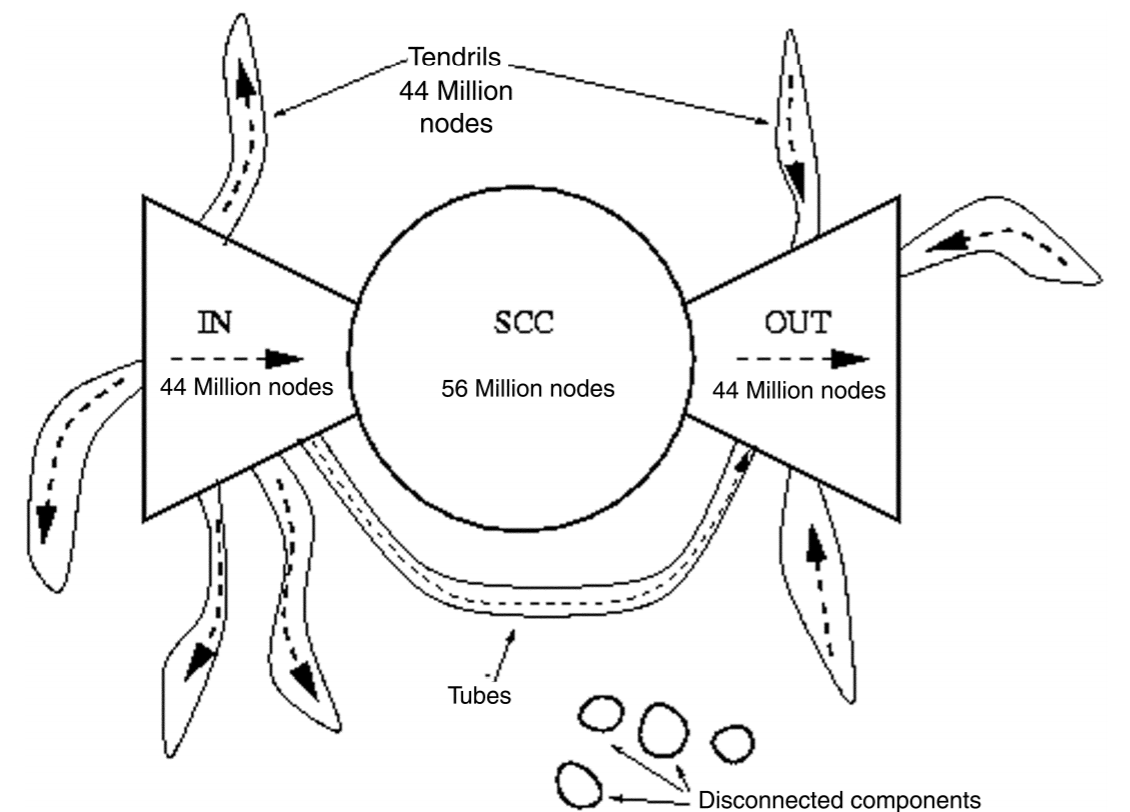
\includegraphics[width=0.45\columnwidth]{web_bowtie.png}
  \caption{Bowtie structure of the web, as described in Broder et al., showing SCC, IN, OUT, TENDRILS, TUBES and DISCONNECTED components of the graph.}
  \label{fig:bowtie}
\end{figure}

\subsection{Node Position [5 points]}

Using outgoing BFS (breadth first search following outgoing edges from a given node) and incoming BFS (the same, but using incoming edges to a given node), how would you determine whether a given node lies in SCC, IN or OUT?

Consider the node with ID 2018 in the Email graph, and the node with ID 224 in the Epinions graph. Run outgoing BFS and incoming BFS on these two nodes (in their respective graphs) and determine whether they lie in SCC, IN or OUT. 

\subsection{Random-start BFS [8 points]}
For each of the two networks, choose 100 nodes at random and do one forward and one backward BFS traversal for each node.  For each direction, make a list containing the number of nodes reachable from each of your 100 random nodes. Sort this list. For each item in the sorted list, plot the index in the list on the x axis, and the value on the y axis. Normalize the x axis so it goes from 0 to 1. The result is a plot like in the paper by Broder et al. (Figure~\ref{fig:ins} below), which shows what percentage of nodes have a reachable tree smaller than a given size. Create one figure for the forward BFS and one for the backward BFS (you should have a total of 4 figures, 2 for each network). Based on the figures, what can you say about the relative size of SCC, IN and OUT in each network? Explain in a few lines. 

\begin{figure}[!htb]
\centering
  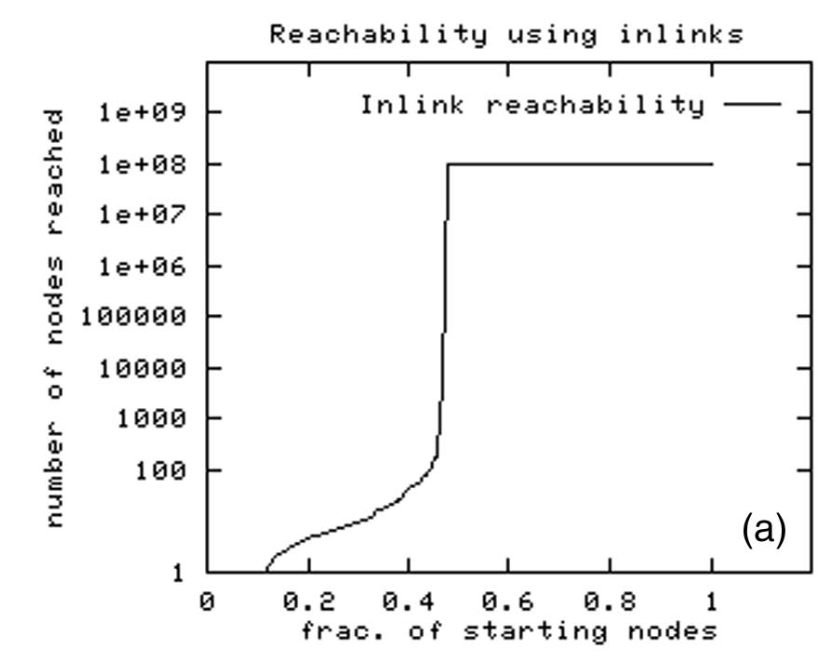
\includegraphics[width=0.45\columnwidth]{in.png}
  \caption{Cumulative distribution on the number of nodes reached by incoming BFS started from randomly chosen nodes.}
  \label{fig:ins}
\end{figure}

\subsection{Size of Bowtie Regions [7 points]}
Describe the behavior you see in each of the 4 above graphs, and what that tells you about the two networks. Try to determine the sizes of each region in the network. How many nodes are in the SCC, IN, OUT, TENDRILS+TUBES (referring to TENDRILS and TUBES combined), and DISCONNECTED regions of each of the two networks? Describe how you calculate the size of each of the above components in a few lines. (\textit{Hint}: You may want to use the SNAP functions \texttt{GetMxWcc} and \texttt{GetMxScc} along with BFS.) 

\subsection{Probability of a Path Existing Between Two Randomly Chosen Nodes [5 points]}
Broder et al. found in their paper that given a pair of randomly chosen start and finish webpages, one can get from the start page to the finish page by traversing links only approx 25\% of the time. \\
For each of the Epinions and the Email networks, what is the probability that a path exists between two nodes chosen uniformly from the graph? \\
As the number of node pairs sampled grows larger, what would you expect the fraction of reachable pairs to converge to, as a function of the sizes of SCC, IN, and OUT? Assume TUBES, TENDRILS, and DISCONNECTED all have negligible size in your expression.


\subsection*{What to submit}
\begin{enumerate}[{Page} 1:]
\setcounter{enumi}{3}
\item 
\begin{itemize}
\item Explanation for how to determine whether a node lies in SCC, IN or OUT
\item For each of the two nodes, whether they lie in SCC, IN or OUT
\end{itemize}

\item
\begin{itemize}
\item Four plots (cumulative number of nodes reached for incoming and outgoing BFS for each of two networks)
\item 1-2 sentence explanation (in terms of relative sizes of SCC, IN and OUT) of the observed BFS traversal behavior
\end{itemize}

\item
\begin{itemize}
\item Size of SCC, IN, OUT, TENDRILS+TUBES, DISCONNECTED regions for each of the two graphs
\item Explanation for how you computed the size of each component
\end{itemize}

\item 
\begin{itemize}
\item Results of experiments performed on at least 100 nodes: probability of a path existing between a pair of nodes chosen from the entire graph, for each of the two networks.
\item 1-2 sentence explanation on expected probability as number of sampled nodes grows large.
\end{itemize}
\end{enumerate}

\newpage

% Q2
% !TEX root = hw1.tex

\section{Link Analysis [25 points]}

\subsection{Personalized PageRank I [12 points]}
Personalizing PageRank is a very important real-world problem: different users
find different pages relevant, so search engines can provide better results if
they tailor their page relevance estimates to the users they are serving. Recall
from class that PageRank can be specialized with clever modifications of the
teleport vector. In this question, we will explore how this can be applied to
personalize the PageRank algorithm.

Assume that people's interests are represented by a set of representative
pages. For example, if Zuzanna is interested in sports and food, then we could
represent her interests with the set of pages $\{$\texttt{www.espn.com},
\texttt{www.epicurious.com}$\}$. For notational convenience, we will use
integers as names for webpages.

Suppose you have already computed the personalized PageRank vectors for the following users:
\vspace{-0.25cm}
\begin{itemize}\setlength\itemsep{0pt}
\item Agatha, whose interests are represented by the teleport set $\{1,2,3\}$
\item Bertha, whose interests are represented by the teleport set $\{3,4,5\}$
\item Clementine, whose interests are represented by the teleport set $\{1,4,5\}$
\item Dolo, whose interests are represented by the teleport set $\{1\}$
\end{itemize}

Assume that the weights for each node in a teleport set are uniform.  Without
looking at the graph, can you compute the personalized PageRank vectors for the
following users? If so, how? If not, why not? Assume a fixed teleport parameter
$\beta$.

\vspace{-0.25cm}
\begin{enumerate}[i.]
\item \textbf{[4 points]} Eloise, whose interests are represented by the teleport set $\{2\}$.

\item \textbf{[4 points]} Felicity, whose interests are represented by the teleport set $\{5\}$.

\item \textbf{[4 points]} Glynnis, whose interests are represented by the teleport set $\{1,2,3,4,5\}$ with weights 0.1, 0.2, 0.3, 0.2, 0.2, respectively.
\end{enumerate}

\subsection{Personalized PageRank II [5 points]}

Suppose that you've already computed the personalized PageRank vectors of a set
of users (denote the computed vectors $V$). What is the set of all personalized
PageRank vectors that you can compute from $V$ without accessing the web graph?

\subsection{A different equation for PageRank [8 points]}
In class you that the PageRank equation can be written in different ways. You will prove this in this question.
Recall that the PageRank equation is:
\begin{align}
\label{equation:PageRank}
    \mathbf{r} = \mathbf{A} \mathbf{r},
\end{align}
where $\mathbf{r} \in \mathbb{R}^N$ is the PageRank vector, i.e. the vector of PageRank scores for each of the $N$ nodes, and (where $\mathbf{1}$ is the all-ones column vector of length $N$):
\begin{align}
    \mathbf{A} = \beta \mathbf{M} + \frac{1-\beta}{N}\mathbf{1}\mathbf{1}^\top.
\end{align}
Recall that here, $\mathbf{M}$ is the stochastic adjacency matrix, defined as
\begin{align}
    \mathbf{M}_{ij} = \left\{\begin{array}{lr}
        \frac{1}{d_j} , & \text{if (j,i) is an edge}\\
        0               & \text{otherwise}
        \end{array}\right\}
\end{align}
where $d_j$ is the degree of node $j$. Assume every node has degree at least 1.

Prove that (\ref{equation:PageRank}) is equivalent to
\begin{align}
    \mathbf{r} = \beta\mathbf{M} \mathbf{r}  + \frac{1-\beta}{N}\mathbf{1}.
\end{align}

Hint: Recall that $\mathbf{r}$ is normalized, i.e. $\sum_{i=1}^N \mathbf{r}_i = 1$.

\subsection*{What to submit}
\begin{enumerate}[2.1:]
\setcounter{enumi}{0}
\item
  \begin{itemize} \item  For each of $(i)$,$(ii)$, and $(iii)$, `yes' or `no' and a brief explanation of why or why not. \end{itemize}
  
\item
  \begin{itemize} \item A mathematical expression for the set in terms of $V$ and a brief explanation. \end{itemize}
  
\item
  \begin{itemize} 
  \item Proof that the two PageRank equations are equivalent.
  \end{itemize}

\end{enumerate}

\newpage

% Q3
% !TEX root = hw2.tex

\section{Decision-based Cascades: A Local Election [25 points]}
It's election season and two candidates, Candidate A and Candidate B, are in a
hotly contested city council race in sunny New Suburb Town. You are a strategic
advisor for Candidate A in charge of election forecasting and voter acquisition
tactics.

Based on careful modeling, you've created two possible versions of the social
graph of voters. Each graph has 10,000 nodes, where nodes are denoted by an
integer ID between 0 and 9999.  The edge lists of the graphs are provided in 
the homework bundle.
Both graphs are \textbf{undirected}.

Given the hyper-partisan political climate of New Suburb Town, most voters have
already made up their minds: 40\% know they will vote for A, 40\% know they will
vote for B, and the remaining 20\% are undecided. Each voter's support is
determined by the last digit of their node id. If the last digit is 0--3, the
node supports A. If the last digit is 4--7, the node supports B. And if the last
digit is 8 or 9, the node is undecided.

The undecided voters will go through a 10-day decision period where they choose
a candidate each day based on the majority of their friends. The \textbf{decision period}
works as follows:
\begin{enumerate}
\item The graphs are initialized with every voter's initial state ($A$, $B$, or
  undecided).
\item In each iteration, every undecided voter decides on a candidate.
  Voters are processed in increasing order of node ID.  
  For every undecided voter, if
  the majority of their friends support A, they now support A. If the majority of
  their friends support B, they now support B. ``Majority'' for A means that
  strictly more of their friends support A than the number of their friends supporting B,
  and vice versa for B (ignoring undecided friends).
\item If a voter has an equal number of friends supporting A and B, we assign support
for A or B in alternating fashion, starting with A.  
In other words, as the voters
are being processed in increasing order of node ID, the first tie leads to
support for A, the second tie leads to support for B, the third for A, the fourth for B, and so on.
This alternating assignment happens at a \textit{global level} for the whole network, across all rounds.
(Keep a single global variable that keeps track of whether the current
  alternating vote is A or B, and initialize it to A in the first round. Then as
  you iterate over nodes in order of increasing ID, whenever you assign a vote
  using this alternating variable, change its value afterwards.)
\item When processing the updates, use the values from the current iteration.
  For example, when updating the votes for node 10, you should use the updated
  votes for nodes 0--9 from the current iteration, and nodes 11 and onwards from the
  previous iteration.
\item There are 10 iterations of the process described above.
\item On the 11th day, it's election day, and the votes are counted.
\end{enumerate}

\emph{Note that only the undecided voters go through the decision process. The decision process does not change the loyalties of those voters who have already made up their minds. Voters who are initially undecided may change their mind on each iteration of this process.}

\subsection{Basic Setup and Forecasting [4 points]}
Start your work with the starter code provided.
Read in the two graphs and assign the initial vote configurations to the
network.  Then, perform the 10 iterations of the voting process.  Which candidate wins in
Graph 1, and by how many votes? Which candidate wins in Graph 2, and by how many
votes?

For sanity check, neither of these two numbers (how many votes) is larger than 300.

\subsection{TV Advertising [8 points]}
You have amassed a substantial war chest of \$9000, and you have decided to
spend this money by showing ads on the local news. Unfortunately, only 100 New
Suburb Townians watch the local news---those with ids 3000--3099.  However, your
ads are extremely persuasive, so anyone who sees the ad is immediately swayed to
vote for candidate A regardless of his/her previous decision.  You may spend
\$1000 at a time on ads.  The first \$1,000 reaches voters 3000--3009, the
second \$1000 reaches voters 3010--3019, and so on. In other words, the total of \$$k$ in advertising would reach voters with ids from 3000 to $3000 + \frac{k}{100} - 1$.  This advertising happens
before the decision period.  \emph{After voters are persuaded by your ads, they
  never change their minds again.}

Simulate the effect of advertising spending on the two possible social
graphs. First, read in the two graphs again and assign the initial
configurations as before. Now, before the decision process, you purchase \$$k$
of ads and go through the decision process of counting votes.

For each of the two social graphs, plot \$$k$ (the amount you spend) on the
x-axis (for values $k = 1000, 2000, \ldots, 9000$) and the number of votes for A minus the number of votes for B on the y-axis.  Put these on the
same plot.  What's the minimum
amount you can spend to win the election in each of the two social graphs?

\emph{Note that the TV advertising affects all of the voters who see the ads and not just those who
  are undecided.}

\subsection{Wining and Dining the High Rollers [8 points]}
\label{cascades_3}
TV advertising is only one way to spend your campaign war chest.  You have
another idea to have a very classy \$1000 per plate event for the high rollers
of New Suburb Town (the people with the highest degree in the social graph). You
invite high rollers in order of how many people they know, and everyone that
comes to your dinner is \emph{instantly persuaded to vote for candidate A
  regardless of his/her previous decision}.  
For each high roller you spend \$1000 to this persuasion.  
This event will happen before the
decision period. When there are ties between voters with the same degree, the
high roller with lowest node ID get chosen first.

Simulate the effect of the high roller dinner on the two graphs. First, read in
the graphs and assign the initial configuration as before. Now, before the
decision process, you spend \$$k$ on the fancy dinner and then go through the
decision process of counting votes.

For each of the two social graphs, plot \$$k$ (the amount you spend) on the
x-axis (for values $k = 1000, 2000, \ldots, 9000$) and the number of votes you
win by on the y-axis (that is, the number of votes for A less the number of votes for B).
What's the minimum amount you can spend to win the election in each of the two social graphs?

\emph{Note that wining and dining sways all the voters to vote for A and not
  just those who are undecided.}

\subsection{Analysis [5 points]}
Plot the degree distributions on a log-log scale of the two graphs on the same
plot (as in Question 1.1 on Problem Set 1).  Although both graphs have roughly
the same number of edges, degree distributions are actually very different.
In 1--2 sentences, briefly
summarize how this difference explains the results of 
Question \ref{cascades_3}.

\subsection*{What to submit}
\begin{enumerate}[{Page} 1:]
\setcounter{enumi}{8}
\item 
\begin{itemize}
\item Which candidate wins and by how many votes in each graph.
\end{itemize}
 
\item
\begin{itemize}
\item Plot of winning margin in each graph as a function of \$k (on the same plot)
\item The minimum amount you can spend to win the election in each graph
\end{itemize}
 
\item
\begin{itemize}
\item Plot of winning margin in each graph as a function of \$k (on the same plot)
\item The minimum amount you can spend to win the election in each graph
\end{itemize}
 
\item
\begin{itemize}
\item Log-log plot of the degree distributions (on the same plot),
\item 1--2 sentences on why the plot explains the results of Question \ref{cascades_3}.
\end{itemize}
\end{enumerate}

\newpage

% Q4
% !TEX root = hw3.tex

\section{Influence Maximization [25 points]}

In class we discussed the influence maximization problem and the greedy hill-climbing approach to solving it. In the algorithm, we add nodes to the current seed set one at a time. At step 0, we have an empty set $S_0$. At step $i > 0$, we pick the node which maximizes the marginal gain: $S_i = S_{i-1} \cup \left\{ \arg \max_u f(S_{i-1} \cup \{u\})-f(S_{i-1})\right\}$, where $f(S)$ denotes the number of nodes influenced by the initially active set $S$ (includes the set $S$ itself).

As we showed in  class the hill climbing algorithm cannot guarantee an optimal solution. In other words, there might exist a set $T$ with $|T| = i$ such that $f(S_i) < f(T)$. It is also known that the greedy algorithm is a $(1-(1-\frac{1}{k})^k)$ - approximation for the influence maximization problem (its sub-optimality is bounded). In other words, for every $k \geq 1$, the greedy hill-climbing algorithm outputs a set $S_k$ such that $f(S_k) \geq (1-(1-\frac{1}{k})^k) f(T)$ where T is the optimal set for influence maximization.  

Parts 1 and 2 of this problem ask you to construct examples where the greedy hill climbing returns a sub-optimal solution. In part 2, you will explore examples close to the non-optimal bound for the greedy algorithm for $k=3$. Your answer should consist of: (1) For every node $u$ its influence set $X_u$ (you can describe the set or draw a directed graph where an edge from $A$ to $B$ indicates that node $A$ influences node $B$ with probability $1$),
(2) $S_i$, the set of nodes that a greedy hill climbing would choose after $i$ iterations, and (3) $T$, the optimal set of $i$ nodes.



For all the questions, you can assume: (1) The nodes in $S$ are influencing themselves, i.e., the count of total influence $f(S)$ includes the nodes in $S$. (2) The influence set $X_{u}$ contains all nodes that are influenced by node $u$, both directly and eventually. (3) When several nodes have the same level of marginal gain, we choose one of them at random.\\

\subsection{Non-Optimal Hill-Climbing [8 points]} For $k = 2$, construct an example where $f(S_k) < f(T)$. That is, hill-climbing will only find a non-optimal solution. (Hint: the last step of the greedy approach is optimal given the $k-1$ previous steps.)\\

\subsection{Bounded Non-Optimal Hill-Climbing [8 points]} 


For $k= 3$, construct an example where  $f(S_k) \leq 0.8 f(T)$. That is, hill-climbing will only find a solution that is at most 80\% of the optimal solution.\\
( Note: 0.8 is very close to the true lower bound for $f(S_k)$ when $k=3$ which is approximately 0.70 )

\subsection{Optimality of Hill-Climbing [4 points]} Give a property of influence sets $X_u$ such that $f(S_i) = f(T)$.  In other words, what is a \emph{sufficient} property of influence sets of nodes such that greedy hill-climbing always outputs a set which achieves the maximum possible influence for a set of $i$ nodes? If your condition holds, the algorithm should produce an optimal output for any choice of $i$ between 1 and the number of nodes in the graph. The property does not need to be a necessary one. It must be a property of $X_u$. Properties such as ``the network has only $i$ nodes'' are not valid as correct answers.

There are several correct answers; we will accept all reasonable answers.\\

\subsection{More Hill-Climbing... [5 points]}

Assume that we stop hill-climbing after $k$ steps and $|S_k| = |T| = k$. Recall that in the class we proved a bound in the form of
\begin{equation}
f(T) \leq f(S_k) + \sum_{i=1}^k \delta_i,
\end{equation}
where $ \delta_1, .., \delta_k $ are the largest $k$ values of $f(S_k \cup \{u\}) - f(S_k)$ for any node $u$ in the graph. Construct a family of examples for which $f(S_k) + \sum_{i=1}^k \delta_i - f(T)$ can be arbitrarily large.

To be more specific, given any number $b$ you should exhibit a network (graph) such that $f(S_k) + \sum_{i=1}^k \delta_i - f(T)>b$.

Note: A {\em family} of examples is a set $F$ of examples such that for any number $b$, there exists a network (graph) $E(b) \in F$ (corresponding to $b$) such that $f(S_k) + \sum_{i=1}^k \delta_i - f(T)>b$.

\subsection*{What to submit}
\begin{enumerate}[{Page} 1:]
\setcounter{enumi}{12}
\item
\begin{itemize} \item Submit an example: $X_u$, $S$, $T$. \end{itemize}

\item 
\begin{itemize} \item  Submit an example: $X_u$, $S$, $T$. \end{itemize}

\item 
\begin{itemize} \item Submit a property and a brief explanation. \end{itemize}

\item
\begin{itemize} \item  Submit a family of examples and a brief explanation. \end{itemize}
\end{enumerate}


\end{document}
